\subsection{Package della componente View}
	\begin{figure}[h!]
	\begin{center}
		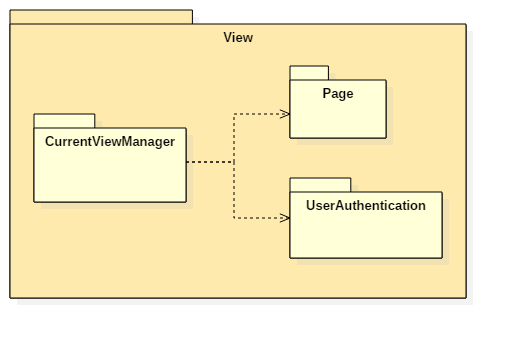
\includegraphics[scale=0.6]{../images/ViewPackage.png}
		\caption{Package della componente View}
	\end{center}
	\end{figure}
	Il package per il componente View del pattern architetturale MVVM contiene i seguenti sotto packages:
	\begin{itemize}
		\item\textbf{Pages:} contiene la classe astratta \textit{Page}, che rappresenta una generica pagina del sistema, più tutte le sue derivazioni concrete, una per ogni pagina prevista. Le pagine possono utilizzare al loro interno dei template per visualizzare situazioni standard gestite da una componente nel package Templates.
		\item\textbf{Templates:} contiene le classi che rappresentano le componenti utilizzabili dalle pagine per visualizzare situazioni o modelli di dati simili tra loro. Si ha così un disaccoppiamento di quali elementi una pagina contiene con come questi sono realizzati.\\
\\
\end{itemize}	